\chapter{The Power of Ambition}

This chapter follows Jim Rohn's lecture as preserved in the curated LazyingArt LLC playlist and keeps its practical order rather than recasting it as a clean institutional course. The formal spine is structural rather than algebraic: definitions, numbered principles, allocation rules, feedback loops, and measurable checkpoints. We begin, as the lecture begins, with a moral restriction. Ambition is powerful only if it works at the service of others and not at their expense, and every later claim about wealth, progress, discipline, and success is filtered through that condition.

\section{Ambition, Greed, and Disciplined Desire}

We do not begin with a neutral dictionary entry. We begin with a boundary. Ambition is legitimate only when it is constructive, when it enlarges life by service, generosity, and discipline rather than by exploitation.

\begin{definition}
Legitimate ambition is ambition at the service of others and not at the expense of others.
\end{definition}

\begin{definition}
True ambition is disciplined eager desire.
\end{definition}

\paragraph{Mechanism.}
Rohn's first formal chain is not symbolic in the usual mathematical sense, but it is exact enough to be written compactly:
\begin{align}
\text{wish} &\longrightarrow \text{desire} \longrightarrow \text{disciplined eager desire} \\
&= \text{ambition} \longrightarrow \text{daily action} \longrightarrow \text{changed life}.
\end{align}
A wish is weak because it asks for the end without consenting to the process. Desire is stronger, but desire still names only what we want. Ambition names the disciplined route by which the wanted end is approached:
\begin{equation}
\text{desire} := \text{the wanted end}, \qquad
\text{ambition} := \text{the disciplined process that reaches it}.
\end{equation}

\paragraph{Illustration.}
The lecture makes the distinction practical at once. If we want to be ready for tomorrow's meeting, we must prepare today. If we want to pay for a child's education, we must save today. If we want a better life tomorrow, we must work on it today. Ambition is therefore not a mood but a repeated present tense.

\subsection{Question \& Answer}

\paragraph{Is ambition just greed in respectable language?}
No. Greed seeks gain by injury, comparison, or manipulation. Ambition, as defined here, is constructive and disciplined. The lecture presses this point through contrast: Judas acquires money, but not success; he gains silver, but not peace. The relevant distinction is not between wanting and not wanting. It is between wanting by destruction and wanting by worthy process. The moral restriction is part of the definition, not an afterthought.

\section{Dreams That Pull and Principles That Organize Life}

Once ambition has been separated from greed, the lecture asks a harder question: what gives disciplined desire enough force to persist? The answer is that wishes remain vague, but dreams can pull.

\paragraph{Mechanism.}
A dream is the projection of the life we want to lead. It becomes effective only when it is vivid:
\begin{equation}
\text{fuzzy future} \Rightarrow \text{little pull}, \qquad
\text{vivid dream} \Rightarrow \text{strong pull}.
\end{equation}
This is why the lecture dwells on pioneers, immigrants, and mountain crossings. The point is not the romance of hardship. The point is that the body can endure a terrible present if the mind sees the finished future in advance.

\paragraph{Illustration.}
To see California while still climbing the mountain, to hear the cheers while still inside the project, to do the uncomfortable until it becomes comfortable: this is the lecture's temporal form of resolve. The word ``until'' does real structural work. It means that the present discomfort does not get a veto over the future.

\paragraph{Structure.}
After the stories, the lecture stabilizes its motivational claims with two numbered schemata. Franklin contributes a three-part pattern:
\begin{equation}
F_{\text{Franklin}} :=
(\text{small daily advantages},
\text{life is moldable},
\text{success as pleasure in present activity}).
\end{equation}
William James contributes a two-part account of success:
\begin{equation}
J_{\text{James}} :=
(\text{inner ideal pursued persistently with courage},
\text{outer achievement related to that ideal}).
\end{equation}
Together they convert atmosphere into method. Great outcomes are built from small daily advantages, and success includes not only attainment but also present right relation to the activity itself.

At this point the lecture presents its main organizing list:
\begin{align}
P_6 := (&\text{positive self-direction},\ \text{self-reliance},\ \text{self-discipline}, \nonumber\\
&\text{self-enterprise},\ \text{working with others},\ \text{self-appreciation}).
\end{align}
What follows is an unpacking of these six principles in order.

\subsection{Question \& Answer}

\paragraph{What turns a wish into a force that can organize a life?}
Three things. First, a vivid image of the end. Second, a principle that breaks the end into daily gains. Third, a temporal vow: we continue until the structure of action becomes stronger than the discomfort of action. This is why the lecture moves from pioneers to Franklin to James. Example first, rule second, persistence always.

\section{Positive Self-Direction: Knowing Ourselves and Preparing Ourselves}

The first principle is positive self-direction. Here the lecture becomes diagnostic. We are asked not merely what we want, but whether our present disciplines are actually carrying us toward it.

\begin{equation}
\text{positive self-direction} := (\text{self-knowledge},\ \text{self-preparation}).
\end{equation}

\begin{proposition}
Direction determines destination.
\end{proposition}

\begin{proof}
The lecture's point is simple. A destination cannot be reached by crossing our fingers while traveling in another direction. Repeated disciplines are steering corrections. If they point elsewhere, they do not accidentally sum to the place we wanted.
\end{proof}

\paragraph{Self-knowledge.}
Self-knowledge means knowing who we are, what we want, what attitudes we have, and what parts of our present life are really ours. The lecture is unusually sharp here. A goal may be admirable and still not be ours. A child may inherit a family career, a family prestige, or a family pressure, and yet be moving toward someone else's destination. The central diagnostic question is therefore not merely, ``Is this a good goal?'' but ``Is it mine?''

\paragraph{Self-preparation.}
Preparation means becoming ready before the opportunity arrives. The lecture turns this into a three-step method:
\begin{enumerate}
\item Identify where the next opportunity is likely to come from.
\item Break preparation for that opportunity into concrete steps.
\item Do additional work to increase the likelihood that the opportunity actually occurs.
\end{enumerate}

Before the figure below, we should be explicit: this is a transcript-derived editorial schematic, not a recovered lecture visual.

\begin{figure}
\centering
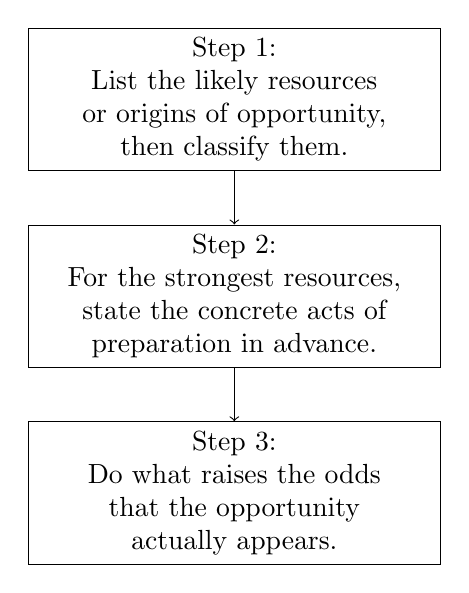
\begin{tikzpicture}
\node[draw, align=center, text width=5.0cm] (a) at (0,0) {Step 1:\\List the likely resources\\or origins of opportunity,\\then classify them.};
\node[draw, align=center, text width=5.0cm] (b) at (0,-2.5) {Step 2:\\For the strongest resources,\\state the concrete acts of\\preparation in advance.};
\node[draw, align=center, text width=5.0cm] (c) at (0,-5.0) {Step 3:\\Do what raises the odds\\that the opportunity\\actually appears.};
\draw[->] (a.south) -- (b.north);
\draw[->] (b.south) -- (c.north);
\end{tikzpicture}
\end{figure}

The lecture even gives a classification vocabulary: some resources are sure things, some good bets, some even chances, some unlikely, and some long shots. The important point is not prediction for its own sake. The point is to convert vague hoping into ranked preparation.

\paragraph{The four ifs.}
The same section compresses a life worth living into four conditions:
\begin{equation}
\text{worthwhile life} := (\text{learn},\ \text{try},\ \text{stay},\ \text{care}).
\end{equation}
This is a strong formal compression. Learning supplies material. Trying tests it. Staying prevents scattered foundations. Caring gives force.

\subsection{Question \& Answer}

\paragraph{Are these goals really mine, or am I living inside someone else's plan?}
The lecture's answer is uncompromising: ask, write, compare, and debate until the goal survives inspection as your own. A noble goal that is alien to the self can still damage the soul. Positive self-direction is not merely aim selection. It is ownership of aim.

\section{Self-Reliance and Self-Discipline as the Missing Link Between Knowledge and Results}

The second and third principles turn from direction to execution. Self-reliance means responsibility. Self-discipline means implementation. Together they answer one of the lecture's most direct questions: if knowledge is power, why do we still fall short?

\paragraph{Self-reliance.}
What happens to us now is, in the lecture's practical sense, connected to what we did yesterday. This does not mean that every circumstance is self-caused. It means that our future will not improve by blame. We may not control wind, season, economy, or the conduct of John in the next office, but we do control preparation, follow-up, reading, study, and skill.

\paragraph{Discipline and procrastination.}
The lecture defines the contrast in near-operational terms:
\begin{equation}
\text{discipline} := \text{awareness of the need for action} + \text{implementation now},
\end{equation}
while
\begin{equation}
\text{procrastination} := \text{delay between awareness and implementation}.
\end{equation}
That is a sharp binary rule. When awareness and action coincide, we have discipline. When a gap opens and we begin saying ``later,'' we have procrastination.

\subsection{Question \& Answer}

\paragraph{If knowledge is power, why do we still fall short?}
Because knowledge without disciplined application produces no harvest. The lecture insists on a sequence: apply what we know, study the results, refine the approach, and apply again. The missing link is not usually more information. It is consistent self-discipline.

\paragraph{Positive reinforcement.}
The lecture repeatedly describes a cumulative loop:
\begin{equation}
\text{disciplined action}
\longrightarrow
\text{small result}
\longrightarrow
\text{encouragement}
\longrightarrow
\text{stronger habit}
\longrightarrow
\text{more disciplined action}.
\end{equation}

\begin{proposition}
Small disciplines are coupled rather than isolated.
\end{proposition}

\begin{proof}
Rohn's examples come as a chain. A daily walk makes right eating easier. Right eating makes reading easier. Reading leads to journaling. Journaling leads to skill development. Thus one discipline affects another. The positive side and the negative side both propagate.
\end{proof}

This is also where the lecture introduces its ``two easies'' formula:
\begin{equation}
\text{easy to do} = \text{easy not to do}.
\end{equation}
The danger is that neglected errors do not look catastrophic on the first day. They drift. Hence the insistence on daily rather than occasional discipline.

\paragraph{Visual chain thinking and the game plan.}
To prevent discouragement, the lecture recommends seeing each task as a link in a chain rather than as an isolated burden. The graph-paper game plan operationalizes this. We place activities against days or time blocks. We do not start the day, the week, or the month until we know its shape. The plan is not merely administrative. It is motivational. It lets the future pull the present.

\section{Self-Enterprise and Working With Others}

The fourth principle is self-enterprise. It is the refusal to wait passively for opportunity. But the lecture immediately refuses to let self-enterprise turn into isolation. Opportunity is created by initiative, yet realized through persons, conversations, trust, and service.

\paragraph{Creativity and courage.}
Self-enterprise requires both. Creativity sees possibility in scrap metal, broken neighborhoods, secondary markets, delayed opportunities, and old problems. Courage permits us to act on what creativity sees. The lecture treats fear, indifference, indecision, doubt, worry, and over-caution as inner enemies precisely because they interrupt this translation from perception to action.

\paragraph{A working problem-solving sequence.}
The lecture offers a compact triad:
\begin{equation}
\text{problem solving} :=
(\text{What can I do?},\ \text{What can I read?},\ \text{Who can I ask?}).
\end{equation}
Again, this is not ornamental. It is an ordered method. We start with present resources, then literature, then counsel.

The following figure is an editorial reconstruction from the transcript.

\begin{figure}
\centering
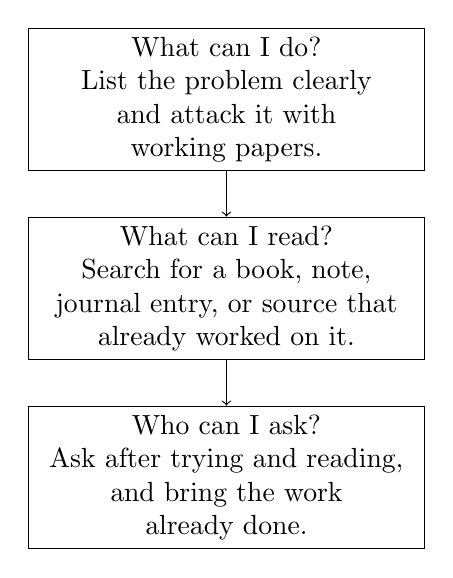
\begin{tikzpicture}
\node[draw, align=center, text width=4.8cm] (a) at (0,0) {What can I do?\\List the problem clearly\\and attack it with\\working papers.};
\node[draw, align=center, text width=4.8cm] (b) at (0,-2.4) {What can I read?\\Search for a book, note,\\journal entry, or source that\\already worked on it.};
\node[draw, align=center, text width=4.8cm] (c) at (0,-4.8) {Who can I ask?\\Ask after trying and reading,\\and bring the work\\already done.};
\draw[->] (a.south) -- (b.north);
\draw[->] (b.south) -- (c.north);
\end{tikzpicture}
\end{figure}

\subsection{Question \& Answer}

\paragraph{How do we create opportunity instead of merely waiting for it?}
We think on paper, we brainstorm, we imagine even outlandish solutions, we use diagrams and doodles to shake thought loose, and we keep learning. Self-enterprise is not mystical luck. It is trained alertness plus repeated initiative.

\paragraph{Working with others.}
The lecture then broadens outward. Kindness, sensitivity, questioning, sincerity, brevity, style, vocabulary, listening, and reading the audience are not decorative skills. They are productive disciplines. A strong business relation, like a strong family relation, is built by communication and maintained by attention.

Several lecture maxims fit here:
\begin{equation}
\text{if you wish to receive} \Rightarrow \text{you must give},
\qquad
\text{if you search} \Rightarrow \text{you will find}.
\end{equation}
And more strongly:
\begin{equation}
\text{if you plant} \Rightarrow \text{you reap},
\qquad
\text{need alone} \not\Rightarrow \text{reap}.
\end{equation}
This is Rohn's language of enlightened self-interest. Service is not loss. Properly understood, it is investment.

\subsection{Question \& Answer}

\paragraph{How can ambition be self-reliant and still depend on other people?}
Because self-reliance is not solitude. It is responsibility for the value we bring to the table. One can count on oneself and still require colleagues, clients, family, mentors, and partners. Indeed, the lecture says it bluntly: it is hard to find a rich hermit. Each of us needs all of us.

\section{Self-Appreciation, Financial Independence, and Measurable Progress}

The sixth principle is self-appreciation. This does not mean vanity. It means acknowledging achievement honestly enough that present gain can fuel future effort. From here the lecture turns toward wealth, money management, and the measurement of progress.

\begin{definition}
Financial independence is the ability to live from the income of one's own personal resources.
\end{definition}

\paragraph{Reward without greed.}
The lecture insists that it is acceptable to want wealth, provided the moral condition is preserved. Wealth is not identified with corruption. Corruption is gain at the expense of others. Wealth, as Rohn presents it, is the reward of disciplined service.

\paragraph{The allocation rule.}
The lecture's most explicit arithmetic prescription is the $70/10/10/10$ rule:
\begin{equation}
\text{spending} \le 0.70Y,\qquad
\text{charity}=0.10Y,\qquad
\text{active capital}=0.10Y,\qquad
\text{passive capital}=0.10Y.
\end{equation}
Here $Y$ denotes income. The point is philosophical before it is financial. We invest first and spend what remains, not the other way around.

\paragraph{Worked example.}
If we take a monthly income of $Y=\$5000$, the lecture's rule becomes
\begin{align}
\text{spending} &\le 0.70Y = \$3500, \\
\text{charity} &= 0.10Y = \$500, \\
\text{active capital} &= 0.10Y = \$500, \\
\text{passive capital} &= 0.10Y = \$500.
\end{align}
Nothing sophisticated is being claimed here beyond disciplined partition. The lecture's point is that repeated right allocation, month after month, changes the future.

\paragraph{Progress by number, not story.}
Rohn then sharpens the lecture into a theory of checkpoints. Progress must be measurable, and the measurement interval must be reasonable:
\begin{equation}
\text{measure of success} := \text{measurable progress in reasonable time}.
\end{equation}
Some things must be checked daily, some weekly, some over ninety days, some over six months. The lecture's sample questions are numerical: how much have we saved and invested, how many books have we read in the last ninety days, how many classes have we taken in the last six months?

A small business example makes the spirit clear. If a new salesperson is supposed to make ten calls in the first week, the relevant measure is
\begin{equation}
n_{\text{calls}}^{\text{target}} = 10, \qquad
n_{\text{calls}}^{\text{actual}} = n.
\end{equation}
By Friday the question is not, ``What is your story?'' It is, ``What is your number?'' The numbers tell the story.

\subsection{Question \& Answer}

\paragraph{Is it acceptable to want wealth, and how do we measure whether we are truly progressing toward it?}
Yes, provided the pursuit remains at the service of others. And we measure progress not by fantasy, not by self-description, and not by borrowed stereotypes, but by numbers taken at proper intervals. Wealth here is not a theatrical symbol. It is disciplined freedom built by allocation, strict accounts, and repeated review.

\section{Failure, Patience, Persistence, and the Final Compression Into Character}

Having discussed reward, the lecture immediately turns to the risk of discouragement. It redefines failure, inserts patience and persistence, and finally compresses the six principles into three cornerstones of character.

\begin{definition}
Success is the steady progress toward one's own personal goals.
\end{definition}

\begin{definition}
Failure is not trying, or no progress because one has ceased to act.
\end{definition}

This is an important reversal. A project that does not work is not yet failure if full effort, learning, and adjustment continue. Failure enters when trying stops.

\subsection{Question \& Answer}

\paragraph{What should we do when progress fails, stalls, or takes much longer than we hoped?}
We do not call the delay final. We study the setback, take responsibility for our part, correct the course, and continue. The lecture's practical answer is patience plus persistence. Delay is not disproof. It is part of the cost.

\paragraph{Patience and persistence.}
The lecture compresses them as follows:
\begin{equation}
\text{persistence} := \text{patience in action}.
\end{equation}
Patience handles the passing of time. Persistence keeps movement alive inside that passing. Together they protect ambition from the false conclusion that delay means defeat.

\paragraph{Resilience.}
Resilience is defined in the lecture through rebound:
\begin{equation}
\text{resilience} := \text{the ability to recover after setback, compression, or adversity}.
\end{equation}
The lecture lists its working components in practical form: insight, independence, ties to others, initiative, creativity, humor, and morality. Especially important is the final term. Rebound is not permitted to become moral collapse. Even recovery must remain at the service of others.

\paragraph{The final compression.}
At the end, the six principles are gathered into three cornerstones:
\begin{align}
P_6 &\longrightarrow C_3, \\
C_3 &:= (\text{concentration},\ \text{resilience},\ \text{integrity}).
\end{align}
Concentration keeps attention fixed on the task at hand. Resilience keeps us moving after setback. Integrity preserves the moral and personal unity of the whole pursuit. The lecture's last great reversal follows immediately: we are more than our ambition. Ambition must serve the self that has been strengthened by these traits, not consume it.

\paragraph{Integrity.}
The most compact formula here is not financial but moral:
\begin{equation}
\text{integrity} \Rightarrow \text{pay fair price for fair value, finish what you begin, keep faith}.
\end{equation}
Integrity is not merely honesty in speech. It is refusal to get something for nothing, refusal to cheat, refusal to leave a task half-done, and refusal to let success be purchased by degradation.

\section{Summary}

The lecture builds ambition from the inside out. First it restricts ambition morally. Then it defines ambition operationally as disciplined eager desire. Then it gives that desire pull by vivid dreams, order by principles, traction by self-direction and self-discipline, inventiveness by self-enterprise, breadth by work with others, and fuel by self-appreciation. Wealth, in this picture, is not a separate topic. It is one domain in which disciplined allocation, service, and measurable progress become visible.

The final compression is the one to remember. The six principles are not six unrelated tips. They are a training ground for concentration, resilience, and integrity. When these are formed, ambition ceases to be a master and becomes an instrument. That is the lecture's closing claim: ambition is powerful, but only when it serves the person who has learned how to direct it, discipline it, moralize it, and sustain it until.